\documentclass[12pt]{article}
\usepackage{../mcm}
\graphicspath{{../images/}}

\begin{document}
\section{Genetic Algorithm}
\subsection{Heat Distribution}
$Fit_{heat}$

\subsection{Packing}
An ideal shape should fill the oven without creating a waste of space, maximizing the number of pans that can fit in the oven.
Clearly, most of the shapes that our GA generates are not able to form tessellations.
As a measure of how well a shape can pack inside the oven, we use the \textit{effective area}.
The effective area is the area where a shape occupies and another shape cannot come in.
For example, if a shape had a hollow circle in the middle, the area would be less than that of the full circle; however, the effective area would be the area of the full circle.
We approximate the effective area $A_{eff}$ by:
\begin{enumerate}
  \item Compute the center of mass, which equals to the mean coordinates of all points.
  \item Consider four quadrants around the mean point.
  \item Within each quadrant, compute the point with the greatest distance from the mean point.
  \item The effective area $A_{eff}$ is approximated by a 4-gon with the four vertices.
  \item The fitness $Fit_{pack}$ is $A/A_{eff}$, a rational number less than or equal to $1$.
\end{enumerate}
The area of a quadrilateral defined by the four edges of length $a,b,c,d$ is computed using the \textit{Bretschneider's formula}.
Fig.~\ref{effarea} shows how a shape with empty areas can have a large effective area.

\begin{equation*}
  \frac{1}{4}\sqrt{4p^2 q^2 - (b^2 + d^2 - a^2 - c^2)^2}.
\end{equation*}
\begin{figure}[t]
  \centering
  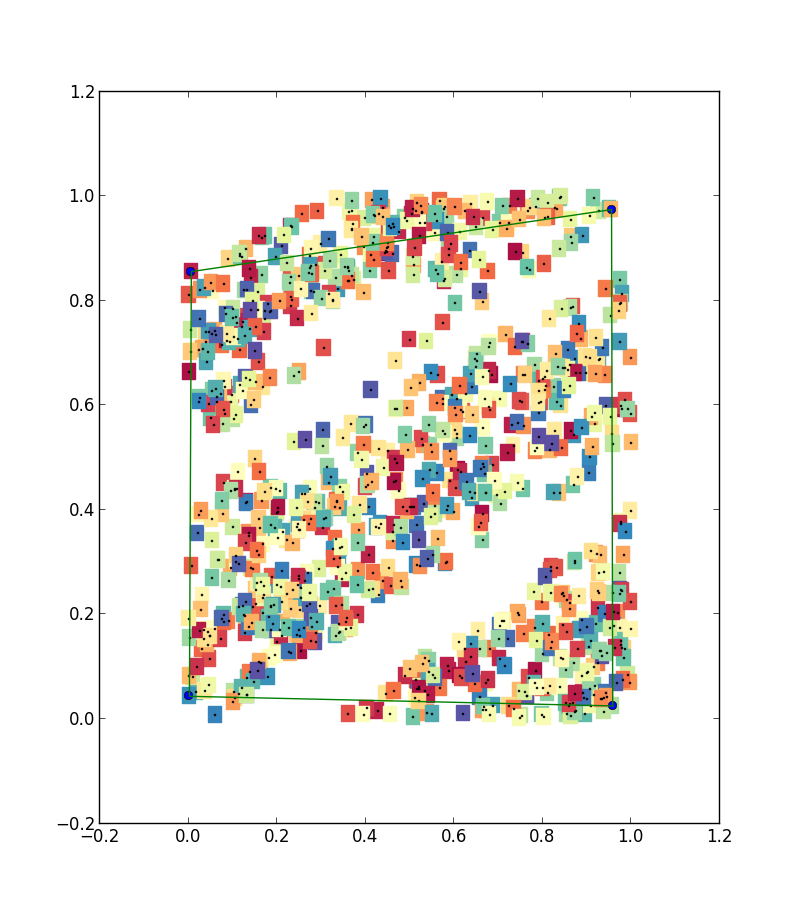
\includegraphics[width=0.6\textwidth]{area_approx}
  \caption{Demonstration of our algorithm to approximate the effective area.
  The area of the square that we started with is 0.81.
  The approximated effective area for this shape is 0.876625844048.}
  \label{fig:effarea}
\end{figure}

\subsection{Balancing The Two}
\end{document}
